\section{Calculated Sum-Frequency Spectra}

One of the aims of this simulation study is to complement our group's previous experimental SFG work.\cite{McFearin2009} The varied set of anions and their affect on the CCl$_4$-H$_2$O interface is linked from theory to empirical data through the connection of computed SFG spectra. The computed SFG spectra for each system are presented in figure \ref{fig:sfg-spectra} along with the experimental spectra from our previous work with these same salt solutions.\cite{McFearin2009} On first look, the overall intensities and lineshapes follow remarkably similar trends as in the experimental systems. The key features of the CCl$_4$-H$_2$O interfacial spectra are the diminished intensities below 3400 cm$^{-1}$ as compared to previous liquid-air works, and the dominant ``free-oh'' peak near 3660 cm$^{-1}$.

\begin{figure}[h!]
\begin{center}
	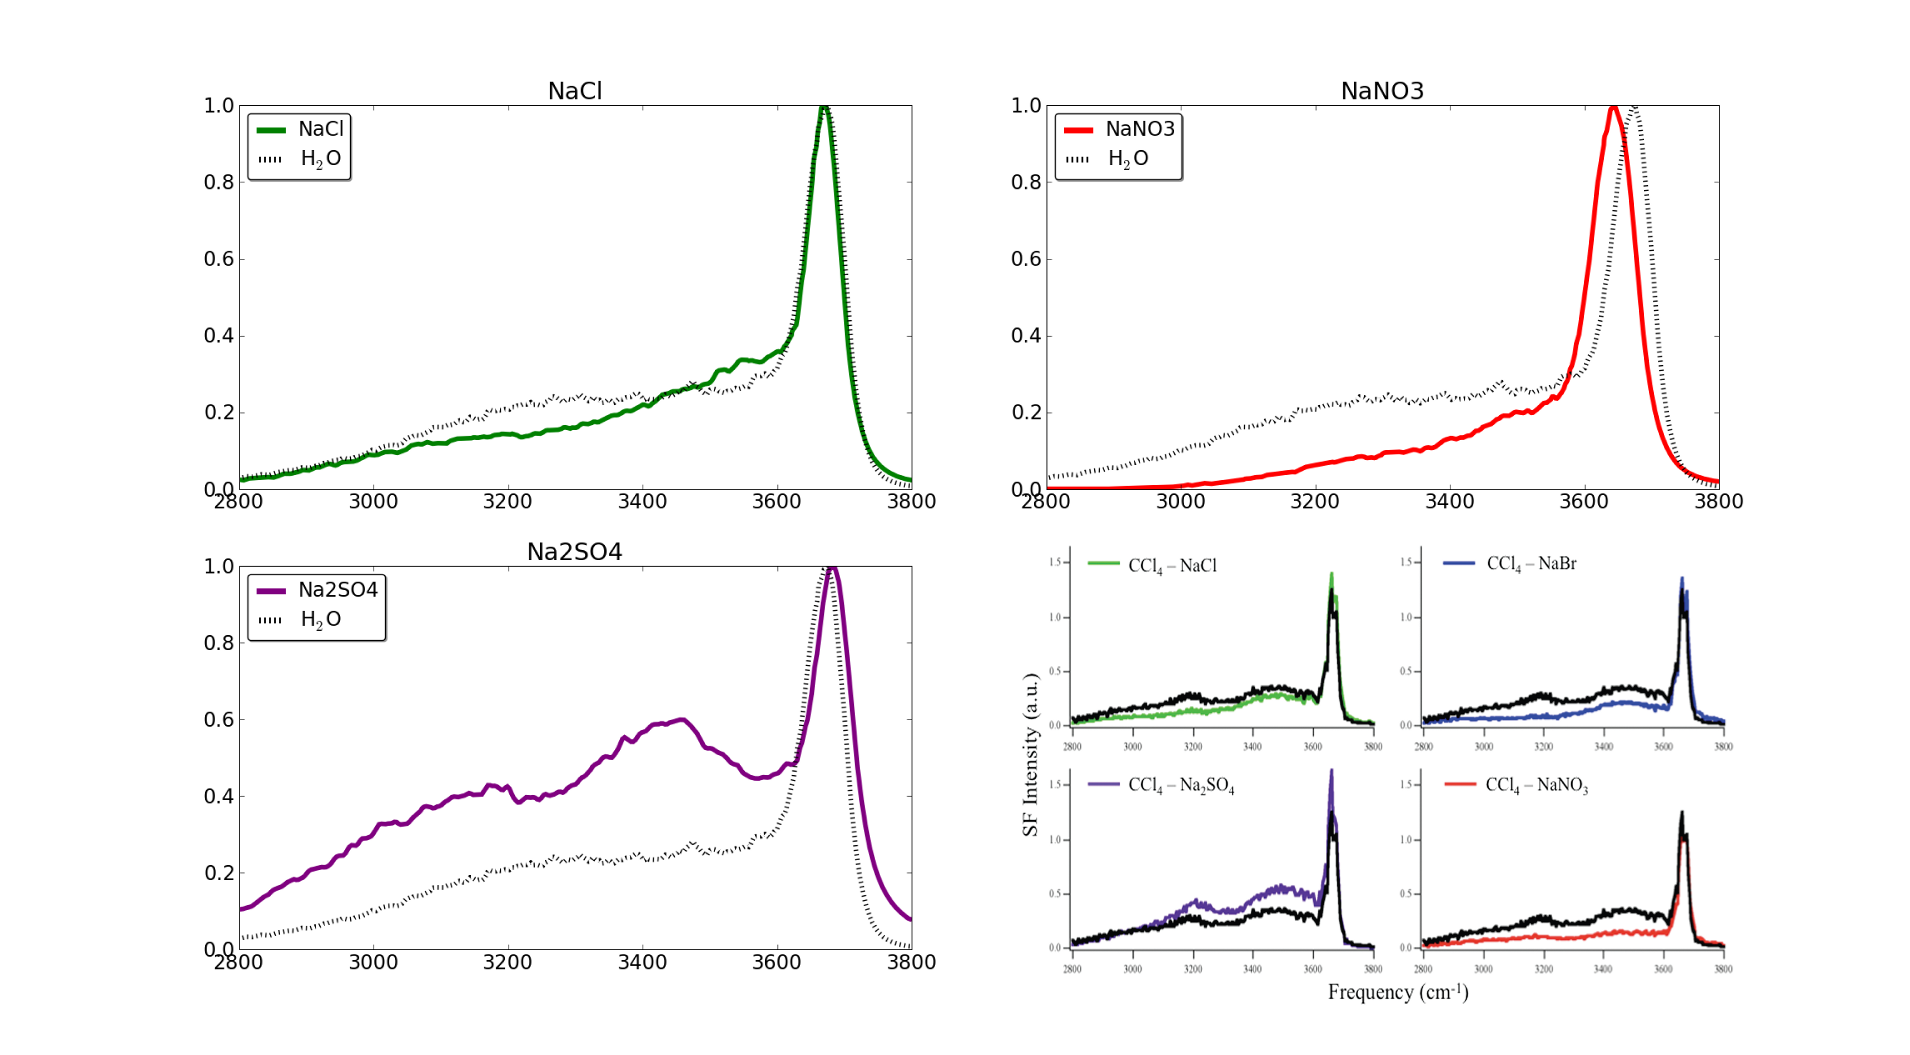
\includegraphics[scale=0.25]{images/sfg-spectra.png}
	\caption{Vibrational SFG spectra of the water-OH stretching region for each interfacial aqueous-salt/CCl$_4$ system. The water/CCl$_4$ interface spectrum (black-dashed line) is provided on the plot for each of the simulated systems for reference. The bottom-right figure is a reproduction of the experimental spectra from McFearin et al to show the intensity and lineshape trends found previously for these systems.\cite{McFearin2009}}
	\label{fig:sfg-spectra}
\end{center}
\end{figure}

The reference CCl$_4$-H$_2$O spectrum reproduces well the lineshape from experiment, but lacks the definition of the two peaks found near 3250 and 3450 cm$^{-1}$. These lower-frequency features have been attributed to the different H-bonding varieties of water that make up the more ``ice-like'' tetrahedral environments found deeper into the aqueous bulk. We have found similar trouble in reproducing the lower-frequency peaks near 3200 cm$^{-1}$, and attribute the slight differences in the lineshape to similar problems.\cite{Walker2006b} However, the lineshape is otherwise quite similar to that of the experiment, and warrants further comparison, and suggests that the methods are sound, and justified for this study.

For monovalent ions at the CCl$_4$-H$_2$O interface, the behavior is completely different than for the air-H$_2$O systems. Previous works found concentrations of monovalent anions to be lower at the CCl$_4$-H$_2$O interface than at the air-liquid one.\cite{Wick2007a} However, larger and more polarizable anions were found to be less solvated than smaller ones such as Cl$^-$, and more surface active.  I$^-$, for instance, has more contact with the CCl$_4$ phase because of a more exposed surface area and higher polarizability, resulting in repulsion of the CCl$_4$, and a wider aqueous interface. The exposure to the CCl$_4$ phase decreases the anion concentration relative to the air-water interface, yet a very prominent density peak remains at the interface for those larger and polarizable ions. The presence of anions at the interface results in a ``field-screening'' that decreases the effect of the changing interfacial field further into the aqeous bulk. Water molecules found below the surface, those giving rise to the lower-frequency 3500 cm$^{-1}$ OH-stretch features, are thus less oriented by the field and their SFG contribution is decreased. Both the monovalent anions, Cl$^-$ and NO$_3^-$, show this effect in their SFG spectra. Comparison to the reference neat-H$_2$O spectrum shows that the added presence of the surface-active anions decreases the lower-frequency intensities, as found in the experimental study. The Cl$^-$ has a notabely smaller decrease in the spectral intensities than the NO$_3^-$ system. This expected result is most likely due to the higher preference for the surface of the larger, and more polarizable nitrate. The NO$_3^-$ ion is extremely surface active, as seen in the density profile, and should thus cause the greatest ``field-screening'' to waters found deeper in the bulk.

The divalent and larger SO$_4^{2-}$ anion accumulates deeper into the aqueous bulk and exhibits the lowest surface affinity of the ions studied. This is likely due to the higher charge of the anion that leads to greater solvation. The sulfate provides little or no screening of the interfacial field from the top-most water layer, and only affects the deeper waters. Lower frequency features of the water OH-spectrum spectrum are noteably higher in intensity and both the 3250 and 3450 cm$^{-1}$ features are present, and dominate as compared to the reference water system, in both the simulated and experimental spectra.

As concluded in the previous experimental work, the monovalent anions appear to screen the deeper water molecules from the field produced by the phase change at the aqueous-organic interface. Larger and more polarizable monovalent anions have a stronger screening effect due to their increased surface affinity. The large but more highly charged divalent anion experiences greater solvation and is thus found deeper in the aqueous phase. Deeper anions do not participate as field screening agents to the same extent as their monovalent counterparts, and the result is an increase across the lower frequencies of the water OH-stretching SFG spectrum.
